\documentclass[mathserif, handout]{beamer}
% ======================================================================
% General LaTeX Setup for Beamer (Reusable Preamble)
% Author: Chandra Gummaluru
% ======================================================================

\documentclass[mathserif, handout]{beamer}
\setbeamertemplate{frametitle}{}

% ------------------------------------------------------------
% basic packages
% ------------------------------------------------------------
\usepackage{url}
\usepackage{ifthen}
\usepackage{enumerate}
\usepackage[font=small]{caption}
\usepackage{subcaption}
\usepackage{moresize}
\usepackage[outline]{contour}
\usepackage{transparent}
\usepackage{worldflags}
\usepackage{bm}
\usepackage{graphbox}
\usepackage{mathtools}
\usepackage{multirow}
\usepackage{fontawesome5}
\usepackage{pifont}
\usepackage{array}
\usepackage{comment}

% ------------------------------------------------------------
% math
% ------------------------------------------------------------
\DeclarePairedDelimiter{\floor}{\lfloor}{\rfloor}
\DeclarePairedDelimiter{\ceil}{\lceil}{\rceil}

% ------------------------------------------------------------
% colors
% ------------------------------------------------------------
\definecolor{hl}{RGB}{248,196,69}
\definecolor{myred}{HTML}{ED5565}
\definecolor{myorange}{HTML}{FC6E51}
\definecolor{myyellow}{HTML}{FFCE54}
\definecolor{mycyan}{HTML}{4FC1E9}
\definecolor{myblue}{HTML}{5D9CEC}

\newcommand{\graytext}[1]{\footnotesize\color{gray}#1\normalsize\color{black}}

% ------------------------------------------------------------
% symbols
% ------------------------------------------------------------
\newcommand{\cmark}{\ding{51}}
\newcommand{\xmark}{\ding{55}}

% ------------------------------------------------------------
% highlighting
% ------------------------------------------------------------
\newcommand{\reducedstrut}{\vrule width 0pt height .9\ht\strutbox depth .9\dp\strutbox\relax}
\newcommand{\highlight}[1]{%
  \begingroup\setlength{\fboxsep}{0pt}\colorbox{hl}{\reducedstrut$\displaystyle #1$\/}\endgroup}
\newcommand{\highlightc}[2]{%
  \begingroup\setlength{\fboxsep}{0pt}\colorbox{#1}{\reducedstrut$\displaystyle #2$\/}\endgroup}

% ------------------------------------------------------------
% environments (boxes)
% ------------------------------------------------------------
\usepackage{tcolorbox}
\tcbuselibrary{skins}

\newtcolorbox{thmbox}[1][]{colback=gray!30!white!20, colframe=black, fonttitle=\bfseries, title=#1, boxrule=0.5pt}

% 1) Bottom open (draw top + sides only)
\newtcolorbox{thmboxtop}[1][]{
    enhanced,
    frame hidden,
    colback=gray!30!white!20,
    borderline north={0.5pt}{0pt}{black}, % top
    borderline west={0.5pt}{0pt}{black},  % left
    borderline east={0.5pt}{0pt}{black}   % right
}

% 2) Top open (draw bottom + sides only)
\newtcolorbox{thmboxbot}[1][]{
    enhanced,
    frame hidden,
    colback=gray!30!white!20,
    borderline south={0.5pt}{0pt}{black}, % bottom
    borderline west={0.5pt}{0pt}{black},  % left
    borderline east={0.5pt}{0pt}{black}   % right
}

% 3) Side only (draw only left and right)
\newtcolorbox{thmboxside}[1][]{
    enhanced,
    frame hidden,
    colback=gray!30!white!20,
    borderline west={0.5pt}{0pt}{black},  % left
    borderline east={0.5pt}{0pt}{black}   % right
}

\newtcolorbox{defboxtop}[1][]{
    enhanced,
    colback=gray!30!white!20,
    frame hidden,
    overlay={
        % Draw top + sides with rounded corners
        \draw[line width=0.5pt, black, rounded corners=3mm]
            (frame.south west) -- (frame.north west) -- (frame.north east) -- (frame.south east);
    },
    #1
}

\newtcolorbox{defboxbot}[1][]{
    enhanced,
    colback=gray!30!white!20,
    frame hidden,
    overlay={
        % Draw top + sides with rounded corners
        \draw[line width=0.5pt, black, rounded corners=3mm]
            (frame.north west) -- (frame.south west) -- (frame.south east) -- (frame.north east);
    },
    #1
}

\newtcolorbox{defboxside}[1][]{
    enhanced,
    frame hidden,
    colback=gray!30!white!20,
    borderline west={0.5pt}{0pt}{black},  % left
    borderline east={0.5pt}{0pt}{black}   % right
}

\newtcolorbox{proofbox}[1][]{colback=gray!20!white!20, colframe=grey, fonttitle=\bfseries, title=#1, boxrule=0.5pt, colbacktitle=white, enhanced jigsaw, sharp corners}

% ------------------------------------------------------------
% code listings
% ------------------------------------------------------------
\usepackage{listings}
\lstdefinestyle{mypython}{
  language=Python,
  deletekeywords=[2]{open, next, from, chr, str, int},
  morekeywords=[3]{List, Graph, Tree, Dict, Set, UnionFind, Ordict, Trie, Queue},
  morekeywords=[4]{ListNode, Vertex, Edge, Path, TreeNode, DictNode, UnifNode, OrdictNode, TrieNode, QueueNode},
  morekeywords=[5]{True, False, Boolean, String, Integer, Key, Function, KeyedObject, Object, Array, Tuple, Optional, None},
  keywordstyle=\color{mycyan}\bfseries,
  keywordstyle=[3]\color{myblue}\bfseries,
keywordstyle=[4]\color{myblue}\bfseries,
keywordstyle=[5]\color{mycyan}\bfseries,
  stringstyle=\color{orange},
  commentstyle=\color{gray}\itshape,
  basicstyle=\ttfamily\footnotesize,
  numbers=left,
  numberstyle=\tiny\color{gray},
  stepnumber=1,
  numbersep=5pt,
  xleftmargin=15pt,
  frame=none,
  showstringspaces=false,
  breaklines=true,
  breakatwhitespace=true,
  tabsize=4,
  columns=flexible
}


% ------------------------------------------------------------
% algorithms
% ------------------------------------------------------------
\usepackage{algorithm}
\usepackage[endLComment=~]{algpseudocodex}
\makeatletter
\algrenewcommand\ALG@beginalgorithmic{\footnotesize}
\makeatother

% ------------------------------------------------------------
% optimization environments
% ------------------------------------------------------------
\usepackage[nocomma]{optidef}

% ------------------------------------------------------------
% pgfplots and pie charts
% ------------------------------------------------------------
\usepackage{pgfplots}
\usepackage{pgf-pie}
\pgfplotsset{compat=1.7}

% ------------------------------------------------------------
% tikz
% ------------------------------------------------------------
\usepackage{tikz}
\usetikzlibrary{
  angles, quotes, positioning, fit, backgrounds, shapes.geometric, intersections,
  calc, shapes, mindmap, decorations.text, arrows, arrows.meta,
  automata, chains, decorations.pathreplacing, calligraphy,
  decorations.markings, shapes.misc, decorations.pathmorphing
}
\tikzset{
  invisible/.style={opacity=0},
  visible on/.style={alt=#1{}{invisible}},
  alt/.code args={<#1>#2#3}{\alt<#1>{\pgfprioritysalso{#2}}{\pgfprioritysalso{#3}}}
}

\newcommand{\multiedge}[5][]{
\pgfmathsetmacro{\N}{#4}
\pgfmathsetmacro{\mid}{(\N-1)/2}
\foreach \i in {0,...,\numexpr#4-1\relax} {

\pgfmathsetmacro{\k}{\i-\mid}
\draw[#1] ($ (#2) + \k*#5*($(#2)!1!90:(#3)$) $) -- ($ (#3) + \k*#5*($(#2)!1!90:(#3)$) $); 

}
\draw[#1,  -{>[scale=1]}]
  ($(#2)!0.54!(#3)$) -- ($(#2)!0.55!(#3)$);
}

% ------------------------------------------------------------
% bibliography
% ------------------------------------------------------------
\usepackage[style=ieee]{biblatex}
\setbeamertemplate{bibliography item}{\insertbiblabel}
\setbeamertemplate{background canvas}{
  \begin{tikzpicture}[remember picture,overlay]
    \node[opacity=0.0075]
      at (current page.center)
      {
\includegraphics[width=0.8\paperwidth]{images/signature.pdf}};
  \end{tikzpicture}
}

% ------------------------------------------------------------
% beamer theme and settings
% ------------------------------------------------------------
\usetheme{Boadilla}
\usecolortheme{seagull}
\beamertemplatenavigationsymbolsempty
\setbeamertemplate{enumerate item}{(\arabic{enumi})}
\setbeamertemplate{enumerate subitem}{(\alph{enumii})}
\setbeamertemplate{enumerate subsubitem}{(\roman{enumiii})}
\setbeamertemplate{itemize item}[circle]
\setbeamertemplate{itemize subitem}{\circ}
\setbeamertemplate{itemize subsubitem}{-}
\setbeamercolor{item}{fg=black!40}
\setbeamercovered{transparent=10}

% ===========================
% Premade TikZ Figure Commands
% ===========================

% images w/ labels
% inside tikz as a node
\NewDocumentCommand{\labeledimgnodetikz}{O{} m m m m m m}{%
	\begin{scope}[transparency group, #1]
		\node[
			draw,
			circle,
			inner sep=0,
			outer sep=0,
			minimum size=10mm,
			#1
		] (#5) at (#3,#4)
		{\includegraphics[scale=#7]{#6}};
		\node[
			rectangle,
			draw=black,
			thick,
			fill=black!55,
			rounded corners=0.1mm,
			inner sep=0pt,
			outer sep=0pt,
			minimum size=2.8mm,
			minimum width=3.5mm
		] at (#3,#4-0.1) {};
		\node[outer sep=0, inner sep=0, white] at (#3,#4-0.1) {\footnotesize #2};
	\end{scope}
}

% inside tikz isolated

% outside tikz
\NewDocumentCommand{\labelednode}{m}{%
	\begin{tikzpicture}[baseline={(0,-1mm)}]
		\node[
			rectangle,
			thick,
			draw=black,
			fill=black!55,
			rounded corners=0.1mm,
			inner sep=0pt,
			outer sep=0pt,
			minimum size=2.8mm,
			minimum width=3.5mm
		] at (0,0) {};
		\node[outer sep=0, inner sep=0, white, minimum size=2.8mm, minimum width=3.5mm] at (0,0) {\footnotesize #1};
	\end{tikzpicture}
}

% images only
% inside tikz as a node
\NewDocumentCommand{\imgnodetikz}{O{} m m m m m m}{%
	\begin{scope}[transparency group, #1]
		\node[
			draw,
			circle,
			inner sep=0,
			outer sep=0,
			minimum size=10mm,
			#1
		] (#5) at (#3,#4)
		{\includegraphics[scale=#7]{#6}};
		\node[
			rectangle,
			draw,
			thick,
			fill=black!55,
			rounded corners=0.1mm,
			inner sep=0pt,
			outer sep=0pt,
			minimum size=2.8mm,
			minimum width=3.5mm,
			opacity=0
		] at (0,0) {};
		\node[outer sep=0, inner sep=0, white, opacity=0] at (0,0) {\footnotesize #2};
	\end{scope}
}

% inside tikz isolated
\NewDocumentCommand{\imgtikz}{O{} mm}{%
	\begin{scope}[transparency group, #1]
		\node[
			inner sep=0,
			outer sep=0
		] (#5) at (#3,#4)
		{\includegraphics[scale=#3]{#2}};
	\end{scope}
}


% outside tikz
\NewDocumentCommand{\imgnode}{mm}{%
	\begin{tikzpicture}[baseline={(0,-1mm)}]
        \node[
            inner sep=0,
            outer sep=0,
            draw opacity=0,
        ] at (0,0)
        {\includegraphics[scale=#2]{#1}};
    \end{tikzpicture}
}

% outside tikz (inline)
\newcommand{\imgnodetext}[2]{%
	\hspace{-0.5mm}%
	\raisebox{-0.26\height}{%
		\includegraphics[scale=#2]{#1}%
	}%
	\hspace{-0.5mm}%
}


% labels only
% inside tikz as a node
\NewDocumentCommand{\labeltikz}{m}{%
	\node[
		rectangle,
		thick,
		draw=black,
		fill=black!55,
		rounded corners=0.1mm,
		inner sep=0pt,
		outer sep=0pt,
		minimum size=2.8mm,
		minimum width=3.5mm
	] at (0,0) {};
	\node[outer sep=0, inner sep=0, white, draw opacity=0] at (0,0) {\footnotesize #1};
}

% inside tikz isolated

% outside tikz

% === define custom pgfkeys ===
\pgfkeys{
	/devicenode/.is family, /devicenode,
	outline thickness/.initial=thick,
	outline color/.initial=black
}

\NewDocumentCommand{\qpacket}{m}{%
	\begin{tikzpicture}[baseline=(current bounding box.center)]
		\node at (0.5,0.4) {\includegraphics[scale=0.1]{#1}};
	\end{tikzpicture}%
}

\NewDocumentCommand{\bpacketid}{mmm}{%
	\begin{tikzpicture}[baseline=(current bounding box.center)]
		\begin{scope}[shift={(0.85,0.7)}]
			\draw[thick, draw=black, fill=#1, rounded corners=1pt] (0.01,0.05) rectangle node[white, text width=1cm, align=center] {\color{#3}\footnotesize #2} (-0.71,-0.625);
		\end{scope}
	\end{tikzpicture}%
}

\NewDocumentCommand{\packetid}{mmmm}{%
	\begin{tikzpicture}[baseline=(current bounding box.center)]
		\begin{scope}[shift={(0.85,0.7)}]
			\draw[thick, draw=black, fill=#2, rounded corners=1pt] (0.01,0.05) rectangle node[white, text width=1cm, align=center] {\color{#4}\footnotesize #3} (-0.71,-0.625);
			\node[
				star,
				star points=30,
				star point ratio=0,
				scale=1.5,
				draw=black,
				thick,
				fill=white,
				rounded corners=0.1mm,
				inner sep=0pt,
				minimum size=2.8mm
			] at (0,0) {};
			\node at (0,0) {\footnotesize #1};
		\end{scope}
	\end{tikzpicture}%
}

\tikzset{
	dictnode/.pic={
			\draw[thick, fill=#1, line join=]
			(-0.75,-0.5) --
			(-0.75,0.5)  --
			(0.75,0.5) --
			(0.75,-0.5) --
			cycle --
			(-0.75, 0.75) --
			(0.75, 0.75) --
			(0.75, -0.5) --
			cycle;
		}
}

\tikzset{
	queuenode/.pic={
			\draw[thick, fill=#1, line join=round]
			(-0.85,-0.5) --
			(-0.85,0.5)  --
			(0.65,0.5) --
			(0.75,0) --
			(0.65,-0.5) --
			cycle;
		}
}

\tikzset{
	queuenodetail/.pic={
			\draw[thick, fill=#1, line join=round]
			(-0.75,-0.5) --
			(-0.75,0.5)  --
			(0.65,0.5) --
			(0.75,0) --
			(0.65,-0.5) --
			cycle;
		}
}

\tikzset{
	listnode/.style={
			shape=rectangle,
			rounded corners,
			thick,
			minimum height=10mm,
			minimum width=15mm,
			inner sep=0pt
		}
}

\tikzset{
	arraynode/.style={
			shape=rectangle,
			thick,
			minimum height=10mm,
			minimum width=15mm,
			inner sep=0pt
		}
}

\tikzset{
	graphnode/.style={
			shape=circle,
			thick,
			minimum size=5mm,
			inner sep=0pt
		}
}

\tikzset{
	defaultnode/.style={
			transform shape,
			circle,
			draw=black,
			thick,
			fill=white,
			minimum size=10mm,
			inner sep=0pt
		},
	newnode/.style={
			transform shape,
			defaultnode,
			draw=myyellow,
			fill=myyellow!60,
			very thick
		},
	newnodelight/.style={
			transform shape,
			defaultnode,
			draw=myyellow,
			fill=myyellow!30,
			very thick
		},
	deletenode/.style={
			defaultnode,
			draw=gray,
			dashed,
			fill=lightgray,
			text=gray,
			very thick
		},
	nooutlinenode/.style={
			defaultnode,
			draw=none,
            draw opacity=0,
			text=black,
			very thick
		},
    nofillnode/.style={
			defaultnode,
			fill=none,
            text=black,
			very thick
		}
}
\tikzset{
	faded/.style={opacity=0.5, text opacity=0.5, transparency group}
}
\tikzset{
	smallgraytext/.style={font=\footnotesize\color{gray}}
}
\tikzset{
	graytext/.style={font=\normalsize\color{gray}}
}
\tikzset{
  squigglearrow/.style={
    very thick,
    lightgray,
    decorate,
    decoration={
      snake,
      amplitude=1.75pt,
      segment length=8pt
    }
  }
}



% title
\title{Tries}
\subtitle{Algorithms and Data Structures}
\author[C. Gummaluru]{Chandra Gummaluru}
\titlegraphic{
\includegraphics[width=0.15\linewidth]{images/signature.pdf}}
\institute[]{\url{chandra-gummaluru.github.io} }
\date[Algorithms and Data Structures]{}

\begin{document}

\begin{frame}
  \maketitle
\end{frame}


\begin{frame}{Motivation}
  \begin{center}
    \Large \highlight{\textbf{motivation}}
  \end{center}
\end{frame}

\begin{frame}
  Devices are typically identified using a number called an \highlight{\textbf{internet}} \highlight{\textbf{protocol (IP) address}}.
  \\~\\
  An IPv4 address is a type of IP address that uses 32-bits: \\
  \begin{center}
    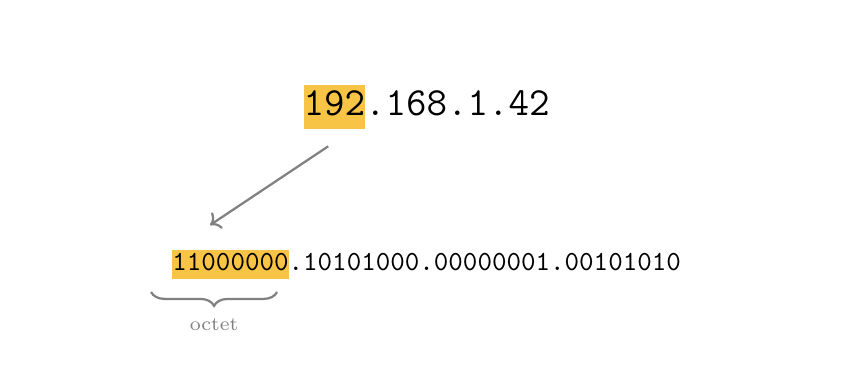
\begin{tikzpicture}
      \draw[opacity=0] (-5,-2) rectangle (5,1);
      \node at (0,0) {\Large \highlight{\texttt{192}}\texttt{.168.1.42}};
      \begin{scope}[yshift=-5mm]
        \draw[thick, ->, gray] (-1.25, 0) -- (-2.75, -1);
      \end{scope}
      \node at (0,-2) {\highlight{\texttt{11000000}}\texttt{.10101000.00000001.00101010}\color{gray}};

      \draw [gray, thick, decorate,decoration={brace,mirror,amplitude=5pt}]
      (-3.5,-2.35) -- ++(1.6,0) node [midway, below=2mm, text width=4.5cm, align=center] {\scriptsize octet};
    \end{tikzpicture}
  \end{center}
  It is usually written in dotted decimal form, with 4 octets of 8 bits each.

\end{frame}

\begin{frame}
  When a device (\imgnodetext{images/server.png}{0.0325}) needs to send a message to another device (\texttt{10.1.1.42}), it must find that device within its routing table.
  \vspace{0.5em}
  \begin{center}
    \begin{tabular}{lc}
      \textbf{Device}         & \textbf{Hop}                               \\
      \hline
      \texttt{10.142.32.81}   & \raisebox{0mm}{\labelednode{\texttt{A}}}   \\
      \texttt{111.122.222.27} & \raisebox{1.5mm}{\labelednode{\texttt{B}}} \\
      \texttt{10.1.1.40}      & \raisebox{1.5mm}{\labelednode{\texttt{C}}} \\
      \hspace{1cm}$\vdots$    &                                            \\
      \texttt{112.12.41.411}  & \raisebox{1.5mm}{\labelednode{\texttt{A}}} \\
    \end{tabular}
  \end{center}
  \vspace{1em}
  However, not all devices will have an entry.
\end{frame}

\begin{frame}
  \vspace{-2mm}
  A \highlight{\textbf{subnetwork}} (or subnet) is a group of devices that share the same IP address prefix, meaning they belong to the same local network range.
  \begin{center}
    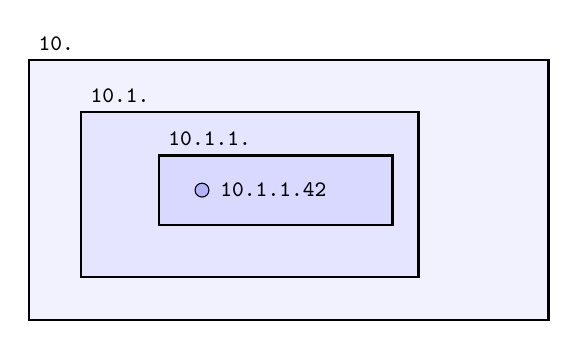
\begin{tikzpicture}[scale=1.1, every node/.style={font=\small}]

      \draw[thick, fill=blue!5] (-3,-1.5) rectangle (3,1.5);
      \node[anchor=south west, font=\footnotesize] at (-3,1.5) {\texttt{10.}};

      \draw[thick, fill=blue!10] (-2.4,-1.0) rectangle (1.5,0.9);
      \node[anchor=south west, font=\footnotesize] at (-2.4,0.9) {\texttt{10.1.}};

      \draw[thick, fill=blue!15] (-1.5,-0.4) rectangle (1.2,0.4);
      \node[anchor=south west, font=\footnotesize] at (-1.5,0.4) {\texttt{10.1.1.}};

      \filldraw[fill=blue!30, draw=black] (-1.0,0.0) circle (0.08);
      \node[anchor=west, font=\footnotesize] at (-0.9,0.0) {\texttt{10.1.1.42}};

    \end{tikzpicture}
    \\[2mm]
    \footnotesize\color{gray}
    Longer prefixes (e.g. \texttt{10.1.1.}) are contained within shorter ones (e.g. \texttt{10.1.}). \\ Each level represents a sub-network within the previous level.
  \end{center}
\end{frame}



\begin{frame}
  When sending a message to a device, the sender (\imgnodetext{images/server.png}{0.0325}) can find the \highlight{\textbf{longest}} \highlight{\textbf{prefix match}} instead.
  \vspace{0.5em}
  \begin{center}
    \begin{tabular}{lc}
      \textbf{Device}              & \textbf{Hop}             \\
      \hline
      \texttt{10.}                 & \labelednode{\texttt{A}} \\
      \texttt{10.1.}               & \labelednode{\texttt{B}} \\
      \highlight{\texttt{10.1.1.}} & \labelednode{\texttt{C}} \\
      \texttt{11.}                 & \labelednode{\texttt{A}} \\
      \hspace{1cm}$\vdots$         &                          \\
    \end{tabular} \\[2mm]
    \footnotesize\color{gray}
    the sender (\imgnodetext{images/server.png}{0.0325}) sends messages to devices within sub-network \texttt{10.1.1.} \\ (such as \texttt{10.1.1.42}) to \labelednode{\texttt{C}}.\color{black}\normalsize
  \end{center}
  One way to find the longest prefix match is to scan every entry and track the longest matching prefix, but this is inefficient.
\end{frame}

\begin{frame}
  \begin{columns}[T]
    \begin{column}{0.48\textwidth}
      \centering
      \begin{tabular}{lc}
        \textbf{Device} & \textbf{Hop}                             \\
        \hline
        \texttt{0}      & \raisebox{0mm}{\labelednode{\texttt{A}}} \\
        \texttt{00}     & \raisebox{0mm}{\labelednode{\texttt{B}}} \\
        \texttt{000}    & \raisebox{0mm}{\labelednode{\texttt{C}}} \\
        \texttt{0001}   & \raisebox{0mm}{\labelednode{\texttt{D}}} \\
        \texttt{01}     & \raisebox{0mm}{\labelednode{\texttt{E}}} \\
        \texttt{1}      & \raisebox{0mm}{\labelednode{\texttt{F}}} \\
        \texttt{10}     & \raisebox{0mm}{\labelednode{\texttt{G}}} \\
        \texttt{1000}   & \raisebox{0mm}{\labelednode{\texttt{I}}} \\
      \end{tabular}
    \end{column}

    \begin{column}{0.48\textwidth}
      \centering
      \begin{tabular}{lc}
        \textbf{Device} & \textbf{Hop}                             \\
        \hline
        \texttt{1001}   & \raisebox{0mm}{\labelednode{\texttt{J}}} \\
        \texttt{101}    & \raisebox{0mm}{\labelednode{\texttt{K}}} \\
        \texttt{1011}   & \raisebox{0mm}{\labelednode{\texttt{L}}} \\
        \texttt{11}     & \raisebox{0mm}{\labelednode{\texttt{M}}} \\
        \texttt{110}    & \raisebox{0mm}{\labelednode{\texttt{N}}} \\
        \texttt{111}    & \raisebox{0mm}{\labelednode{\texttt{O}}} \\
        \texttt{1111}   & \raisebox{0mm}{\labelednode{\texttt{P}}} \\
      \end{tabular}
    \end{column}
  \end{columns}
  \begin{center}
    \graytext{the routing table of a device needing to send a message to \texttt{1010}}
  \end{center}
\end{frame}

\begin{frame}
  \begin{columns}[T]
    \begin{column}{0.48\textwidth}
      \centering
      \begin{tabular}{lc}
        \textbf{Device}                       & \textbf{Hop}                             \\
        \hline
        \texttt{0}                            & \raisebox{0mm}{\labelednode{\texttt{A}}} \\
        \texttt{00}                           & \raisebox{0mm}{\labelednode{\texttt{B}}} \\
        \texttt{000}                          & \raisebox{0mm}{\labelednode{\texttt{C}}} \\
        \texttt{0001}                         & \raisebox{0mm}{\labelednode{\texttt{D}}} \\
        \texttt{01}                           & \raisebox{0mm}{\labelednode{\texttt{E}}} \\
        \highlightc{myyellow!60}{\texttt{1}}  & \raisebox{0mm}{\labelednode{\texttt{F}}} \\
        \highlightc{myyellow!60}{\texttt{10}} & \raisebox{0mm}{\labelednode{\texttt{G}}} \\
        \texttt{1000}                         & \raisebox{0mm}{\labelednode{\texttt{I}}} \\
      \end{tabular}
    \end{column}

    \begin{column}{0.48\textwidth}
      \centering
      \begin{tabular}{lc}
        \textbf{Device}                     & \textbf{Hop}                             \\
        \hline
        \texttt{1001}                       & \raisebox{0mm}{\labelednode{\texttt{J}}} \\
        \highlightc{myyellow}{\texttt{101}} & \raisebox{0mm}{\labelednode{\texttt{K}}} \\
        \texttt{1011}                       & \raisebox{0mm}{\labelednode{\texttt{L}}} \\
        \texttt{11}                         & \raisebox{0mm}{\labelednode{\texttt{M}}} \\
        \texttt{110}                        & \raisebox{0mm}{\labelednode{\texttt{N}}} \\
        \texttt{111}                        & \raisebox{0mm}{\labelednode{\texttt{O}}} \\
        \texttt{1111}                       & \raisebox{0mm}{\labelednode{\texttt{P}}} \\
      \end{tabular}
    \end{column}
  \end{columns}
  \begin{center}
    \footnotesize\color{gray} \highlightc{myyellow!60}{\textsf{matching prefixes}} and \highlightc{myyellow}{\textsf{longest matching prefix}}
  \end{center}
\end{frame}

\begin{frame}
  If the routing table is represented using a special structure, finding the longest prefix match becomes easier: \\
  \begin{figure}
    \centering
    \begin{tikzpicture}[scale=0.8, transform shape]
      % Root
      \node[defaultnode] (n1) at (0,0) {$\varnothing$};

      % Level 1
      \labeledimgnodetikz[defaultnode]{\footnotesize\texttt{A}}{-3}{-1.5}{n0}{images/radio_tower.png}{0.044};
      \labeledimgnodetikz[newnodelight]{\footnotesize\texttt{F}}{3}{-1.5}{n1a}{images/radio_tower.png}{0.044};

      % Level 2 (left branch)
      \labeledimgnodetikz[defaultnode]{\footnotesize\texttt{B}}{-5}{-3}{n00}{images/radio_tower.png}{0.044};
      \labeledimgnodetikz[defaultnode]{\footnotesize\texttt{E}}{-1}{-3}{n01}{images/radio_tower.png}{0.044};

      % Level 2 (right branch)
      \labeledimgnodetikz[newnodelight]{\footnotesize\texttt{G}}{1}{-3}{n10}{images/radio_tower.png}{0.044};
      \labeledimgnodetikz[defaultnode]{\footnotesize\texttt{M}}{5}{-3}{n11}{images/radio_tower.png}{0.044};

      % Level 3 (right -> left branch)
      \node (n100) at (0,-5) [thick, circle, black, draw, minimum width=1cm, minimum height=8mm] {$\varnothing$};
      \labeledimgnodetikz[newnode]{\footnotesize\texttt{K}}{2}{-5}{n101}{images/radio_tower.png}{0.044};
      \labeledimgnodetikz[defaultnode]{\footnotesize\texttt{C}}{-6}{-5}{n000}{images/radio_tower.png}{0.044};

      % Level 4 (right -> left -> right branch)
      \labeledimgnodetikz[defaultnode]{\footnotesize\texttt{L}}{3}{-7}{n1010}{images/radio_tower.png}{0.044};
      \labeledimgnodetikz[defaultnode]{\footnotesize\texttt{I}}{-1}{-7}{n1000}{images/radio_tower.png}{0.044};
      \labeledimgnodetikz[defaultnode]{\footnotesize\texttt{J}}{1}{-7}{n1001}{images/radio_tower.png}{0.044};
      \labeledimgnodetikz[defaultnode]{\footnotesize\texttt{D}}{-5}{-7}{n0001}{images/radio_tower.png}{0.044};


      % Edges
      \draw[thick, ->] (n1) -- node[fill=white] {\texttt{0}} (n0);
      \draw[very thick, ->, myyellow] (n1) -- node[fill=white] {\texttt{1}} (n1a);

      \draw[thick, ->] (n0) -- node[fill=white] {\texttt{0}} (n00);
      \draw[thick, ->] (n0) -- node[fill=white] {\texttt{1}} (n01);

      \draw[very thick, ->, myyellow] (n1a) -- node[fill=white] {\texttt{0}} (n10);
      \draw[thick, ->] (n1a) -- node[fill=white] {\texttt{1}} (n11);

      \draw[very thick, ->, myyellow] (n10) -- node[fill=white] {\texttt{1}} (n101);
      \draw[thick, ->] (n10) -- node[fill=white] {\texttt{0}} (n100);

      \draw[thick, ->] (n101) -- node[fill=white] {\texttt{1}} (n1010);

      \draw[thick, ->] (n100) -- node[fill=white] {\texttt{0}} (n1000);
      \draw[thick, ->] (n100) -- node[fill=white] {\texttt{1}} (n1001);

      \draw[thick, ->] (n00) -- node[fill=white] {\texttt{0}} (n000);
      \draw[thick, ->] (n000) -- node[fill=white] {\texttt{1}} (n0001);
    \end{tikzpicture}
  \end{figure}
\end{frame}

\begin{frame}
  \begin{thmbox}
    \begin{center}
      \scalebox{0.75}{\raisebox{-0.3\height}{
\includegraphics[scale=0.05]{images/bulb.png}}}
    \end{center}
    We need a data structure that can quickly retrieve the key associated with the closest key, without searching through all elements.
  \end{thmbox}

\end{frame}


\begin{frame}{Tries}
  \begin{center}
    \Large \highlight{\textbf{tries}} \\[1mm]
    \normalsize\color{gray} stores strings as paths in a tree structure \\[3mm]
  \end{center}
  \begin{figure}
    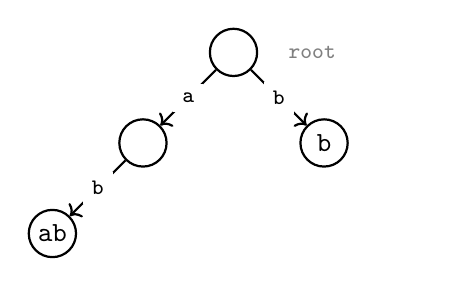
\begin{tikzpicture}
      \tikzset{
        mystyle/.style={
            shape=circle,
            draw=black,
            thick,
            fill=white,
            minimum size=6mm,
            inner sep=0pt
          }
      }
      \node[mystyle] (m1) at (0,0) {$\varnothing$};
      \node[right of =m1, draw=white, xshift=-0mm] {\graytext{\texttt{root}}};
      \node[mystyle] (m2) at (-1.15,-1.15) {$\varnothing$};
      \node[mystyle] (m3) at (1.15,-1.15) {\texttt{b}};
      \node[mystyle] (m4) at (-2.3,-2.3) {\texttt{ab}};
      \node (m5) at (2.3,-2.3) {};
      \draw[thick, ->] (m1) edge node[midway, fill=white] {\footnotesize \texttt{a}} (m2);
      \draw[thick, ->] (m1) edge node[midway, fill=white] {\footnotesize \texttt{b}} (m3);
      \draw[thick, ->] (m2) edge node[midway, fill=white] {\footnotesize \texttt{b}} (m4);
    \end{tikzpicture}
  \end{figure}
\end{frame}

\begin{frame}[fragile]
  A \texttt{Trie} stores \texttt{TrieNode} objects and supports the following operations:\\~\\
  \begin{itemize}

    \item \highlight{\texttt{get}} \\
          \graytext{returns the closest prefix match}\\[-1mm]
          \begin{lstlisting}[style=mypython]
get(key: Key) -> Optional[TrieNode]
\end{lstlisting}

    \item \highlight{\texttt{insert}} \\
          \graytext{inserts an object, creating nodes as needed}\\[-1mm]
          \begin{lstlisting}[style=mypython]
insert(key: Key, obj: Object) -> Optional[TrieNode]
\end{lstlisting}

    \item \highlight{\texttt{delete}} \\
          \graytext{removes an object (if it exists) and extra nodes}\\[-1mm]
          \begin{lstlisting}[style=mypython]
delete(key: Key) -> Optional[TrieNode]
\end{lstlisting}

  \end{itemize}
\end{frame}


\begin{frame}{Tries (via Trees)}
  \begin{center}
    \Large \highlight{\texttt{Trie}} \\[1mm]
    \normalsize \color{gray} (via Trees)
  \end{center}

\end{frame}


\begin{frame}[fragile]
  \begin{thmboxtop}
    \highlight{\texttt{Trie}} \\
    \graytext{(via Trees)}
    \begin{lstlisting}[style=mypython]
class TrieNode:    
    # the object of this node
    obj: Optional[Object]

    # the children of this node
    children: Dict[Key, TrieNode]
\end{lstlisting}
  \end{thmboxtop}
\end{frame}

\begin{frame}[fragile]
  \begin{thmboxbot}
    \begin{lstlisting}[style=mypython]
class Trie:
# attributes 
    # the root
    root: TrieNode

# functions
    ...
\end{lstlisting}
  \end{thmboxbot}
\end{frame}

\begin{frame}
  \begin{center}
    \highlight{\textbf{get}} \\
    \footnotesize\color{gray} \texttt{get(101)}
  \end{center}
  \begin{center}

    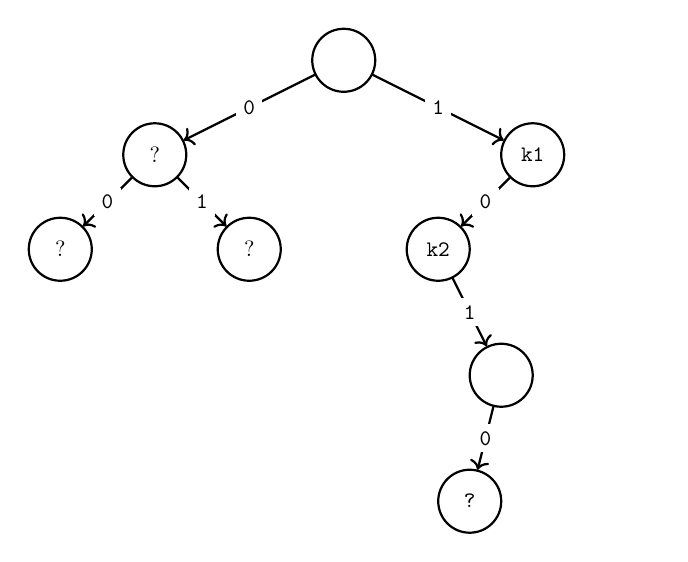
\begin{tikzpicture}[scale=0.8, transform shape]
      \node[defaultnode] (n1) at (0,0)  { $\varnothing$ };
      \node[defaultnode] (n2) at (-3,-1.5)  { ? };
      \node[defaultnode] (n3) at (3,-1.5)  { \texttt{k1} };
      \node[defaultnode] (n4) at (-4.5,-3)  { ? };
      \node[defaultnode] (n5) at (1.5,-3)  { \texttt{k2} };
      \node[defaultnode, opacity=0] (n7) at (4.5,-3)  { \texttt{k} };
      \node[defaultnode] (n8) at (2.5,-5)  { $\varnothing$ };
      \node[defaultnode] (n9) at (2,-7)  { \texttt{?} };
      \node[defaultnode] (n6) at (-1.5,-3)  { ? };

      \draw[thick, ->] (n1) -- node[fill=white] {\texttt{0}} (n2);
      \draw[thick, ->] (n1) -- node[fill=white] {\texttt{1}} (n3);

      \draw[thick, ->] (n2) -- node[fill=white] {\texttt{0}} (n4);
      \draw[thick, ->] (n2) -- node[fill=white] {\texttt{1}} (n6);

      \draw[thick, ->] (n3) -- node[fill=white] {\texttt{0}} (n5);

      \draw[thick, ->] (n5) -- node[fill=white] {\texttt{1}} (n8);
      \draw[thick, ->] (n8) -- node[fill=white] {\texttt{0}} (n9);

    \end{tikzpicture}
  \end{center}
  \begin{center}
    \footnotesize\color{gray} traverse the edges based on the key's characters \\ cache deepest key found thus far
  \end{center}
\end{frame}

\begin{frame}
  \begin{center}
    \highlight{\textbf{get}} \\
    \footnotesize\color{gray} \texttt{get(101)}
  \end{center}
  \begin{center}

    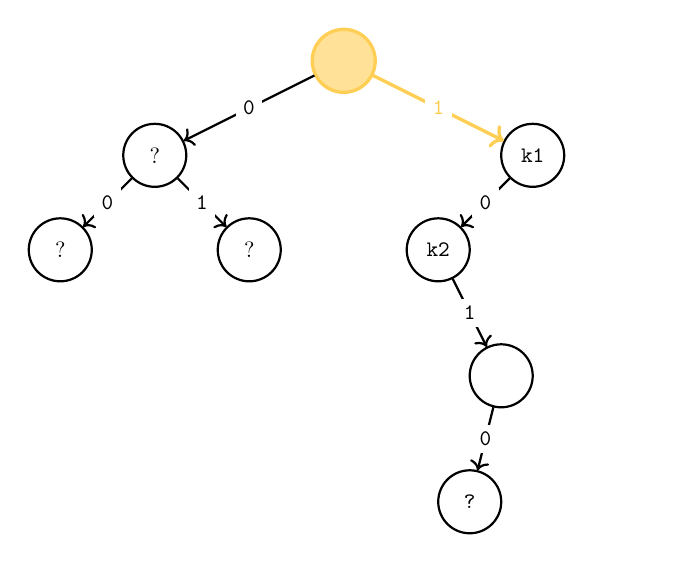
\begin{tikzpicture}[scale=0.8, transform shape]
      \node[newnode] (n1) at (0,0)  { $\varnothing$ };
      \node[defaultnode] (n2) at (-3,-1.5)  { ? };
      \node[defaultnode] (n3) at (3,-1.5)  { \texttt{k1} };
      \node[defaultnode] (n4) at (-4.5,-3)  { ? };
      \node[defaultnode] (n5) at (1.5,-3)  { \texttt{k2} };
      \node[defaultnode, opacity=0] (n7) at (4.5,-3)  { \texttt{k} };
      \node[defaultnode] (n8) at (2.5,-5)  { $\varnothing$ };
      \node[defaultnode] (n9) at (2,-7)  { \texttt{?} };
      \node[defaultnode] (n6) at (-1.5,-3)  { ? };

      \draw[thick, ->] (n1) -- node[fill=white] {\texttt{0}} (n2);
      \draw[very thick, ->, myyellow] (n1) -- node[fill=white] {\texttt{1}} (n3);

      \draw[thick, ->] (n2) -- node[fill=white] {\texttt{0}} (n4);
      \draw[thick, ->] (n2) -- node[fill=white] {\texttt{1}} (n6);

      \draw[thick, ->] (n3) -- node[fill=white] {\texttt{0}} (n5);

      \draw[thick, ->] (n5) -- node[fill=white] {\texttt{1}} (n8);
      \draw[thick, ->] (n8) -- node[fill=white] {\texttt{0}} (n9);

    \end{tikzpicture}
  \end{center}
  \begin{center}
    \footnotesize\color{gray} traverse the edges based on the key's characters \\ cache deepest key found thus far
  \end{center}
\end{frame}

\begin{frame}
  \begin{center}
    \highlight{\textbf{get}} \\
    \footnotesize\color{gray} \texttt{get(101)}
  \end{center}
  \begin{center}

    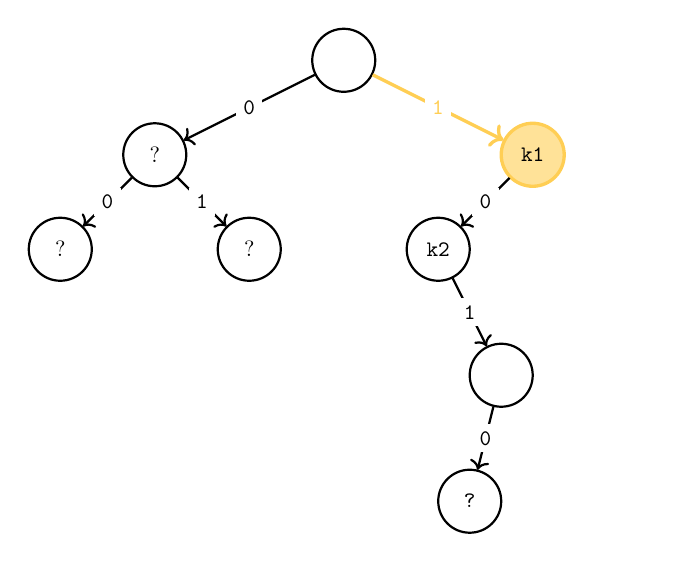
\begin{tikzpicture}[scale=0.8, transform shape]
      \node[defaultnode] (n1) at (0,0)  { $\varnothing$ };
      \node[defaultnode] (n2) at (-3,-1.5)  { ? };
      \node[newnode] (n3) at (3,-1.5)  { \texttt{k1} };
      \node[defaultnode] (n4) at (-4.5,-3)  { ? };
      \node[defaultnode] (n5) at (1.5,-3)  { \texttt{k2} };
      \node[defaultnode, opacity=0] (n7) at (4.5,-3)  { \texttt{k} };
      \node[defaultnode] (n8) at (2.5,-5)  { $\varnothing$ };
      \node[defaultnode] (n9) at (2,-7)  { \texttt{?} };
      \node[defaultnode] (n6) at (-1.5,-3)  { ? };

      \draw[thick, ->] (n1) -- node[fill=white] {\texttt{0}} (n2);
      \draw[very thick, ->, myyellow] (n1) -- node[fill=white] {\texttt{1}} (n3);

      \draw[thick, ->] (n2) -- node[fill=white] {\texttt{0}} (n4);
      \draw[thick, ->] (n2) -- node[fill=white] {\texttt{1}} (n6);

      \draw[thick, ->] (n3) -- node[fill=white] {\texttt{0}} (n5);

      \draw[thick, ->] (n5) -- node[fill=white] {\texttt{1}} (n8);
      \draw[thick, ->] (n8) -- node[fill=white] {\texttt{0}} (n9);

    \end{tikzpicture}
  \end{center}
  \begin{center}
    \footnotesize\color{gray} traverse the edges based on the key's characters \\ cache deepest key found thus far
  \end{center}
\end{frame}


\begin{frame}
  \begin{center}
    \highlight{\textbf{get}} \\
    \footnotesize\color{gray} \texttt{get(101)}
  \end{center}
  \begin{center}

    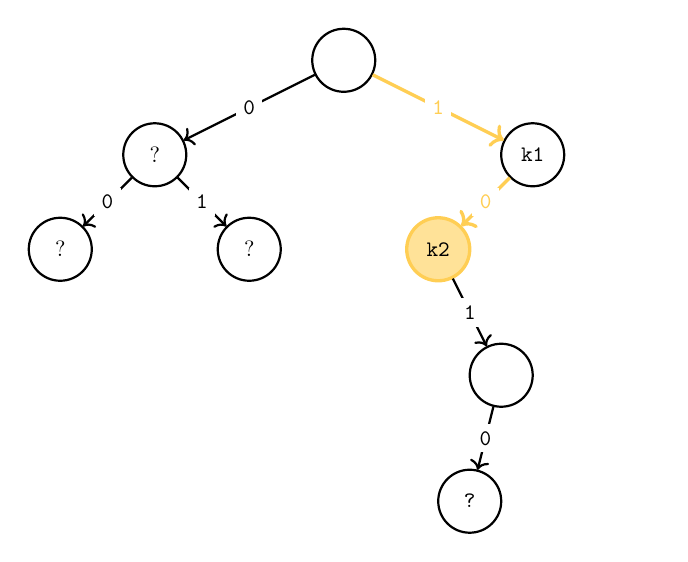
\begin{tikzpicture}[scale=0.8, transform shape]
      \node[defaultnode] (n1) at (0,0)  { $\varnothing$ };
      \node[defaultnode] (n2) at (-3,-1.5)  { ? };
      \node[defaultnode] (n3) at (3,-1.5)  { \texttt{k1} };
      \node[defaultnode] (n4) at (-4.5,-3)  { ? };
      \node[newnode] (n5) at (1.5,-3)  { \texttt{k2} };
      \node[defaultnode, opacity=0] (n7) at (4.5,-3)  { \texttt{k} };
      \node[defaultnode] (n8) at (2.5,-5)  { $\varnothing$ };
      \node[defaultnode] (n9) at (2,-7)  { \texttt{?} };
      \node[defaultnode] (n6) at (-1.5,-3)  { ? };

      \draw[thick, ->] (n1) -- node[fill=white] {\texttt{0}} (n2);
      \draw[very thick, ->, myyellow] (n1) -- node[fill=white] {\texttt{1}} (n3);

      \draw[thick, ->] (n2) -- node[fill=white] {\texttt{0}} (n4);
      \draw[thick, ->] (n2) -- node[fill=white] {\texttt{1}} (n6);

      \draw[very thick, ->, myyellow] (n3) -- node[fill=white] {\texttt{0}} (n5);

      \draw[thick, ->] (n5) -- node[fill=white] {\texttt{1}} (n8);
      \draw[thick, ->] (n8) -- node[fill=white] {\texttt{0}} (n9);

    \end{tikzpicture}
  \end{center}
  \begin{center}
    \footnotesize\color{gray} traverse the edges based on the key's characters \\ cache deepest key found thus far
  \end{center}
\end{frame}


\begin{frame}
  \begin{center}
    \highlight{\textbf{get}} \\
    \footnotesize\color{gray} \texttt{get(101)}
  \end{center}
  \begin{center}

    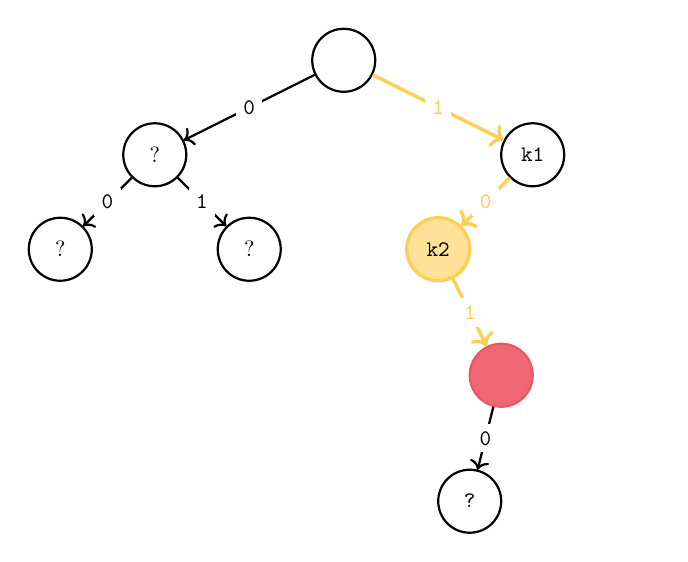
\begin{tikzpicture}[scale=0.8, transform shape]
      \node[defaultnode] (n1) at (0,0)  { $\varnothing$ };
      \node[defaultnode] (n2) at (-3,-1.5)  { ? };
      \node[defaultnode] (n3) at (3,-1.5)  { \texttt{k1} };
      \node[defaultnode] (n4) at (-4.5,-3)  { ? };
      \node[newnode] (n5) at (1.5,-3)  { \texttt{k2} };
      \node[defaultnode, opacity=0] (n7) at (4.5,-3)  { \texttt{k} };
      \node[defaultnode, draw=myred, fill=myred!90] (n8) at (2.5,-5)  { $\varnothing$ };
      \node[defaultnode] (n9) at (2,-7)  { \texttt{?} };
      \node[defaultnode] (n6) at (-1.5,-3)  { ? };

      \draw[thick, ->] (n1) -- node[fill=white] {\texttt{0}} (n2);
      \draw[very thick, ->, myyellow] (n1) -- node[fill=white] {\texttt{1}} (n3);

      \draw[thick, ->] (n2) -- node[fill=white] {\texttt{0}} (n4);
      \draw[thick, ->] (n2) -- node[fill=white] {\texttt{1}} (n6);

      \draw[very thick, ->, myyellow] (n3) -- node[fill=white] {\texttt{0}} (n5);

      \draw[very thick, ->, myyellow] (n5) -- node[fill=white] {\texttt{1}} (n8);
      \draw[thick, ->] (n8) -- node[fill=white] {\texttt{0}} (n9);

    \end{tikzpicture}
  \end{center}
  \begin{center}
    \footnotesize\color{gray} traverse the edges based on the key's characters \\ cache deepest key found thus far
  \end{center}
\end{frame}

\begin{frame}[fragile]
  \begin{proofbox}
    \begin{lstlisting}[style=mypython]        
def get(self: Trie, key: Key) -> Optional[TrieNode]:
    curr = self.root
    longest = None
    for char in key:
        if curr.children[char] is None:
            break
        curr = curr.children[char]
        if curr.obj is not None:
            longest = curr.obj
    return longest
\end{lstlisting}
  \end{proofbox}
\end{frame}

\begin{frame}
  \begin{center}
    \highlight{\textbf{insert}} \\
    \footnotesize\color{gray} \texttt{insert(1010, obj)}
  \end{center}
  \begin{center}

    \begin{tikzpicture}[scale=0.8, transform shape]
      \node[defaultnode] (n1) at (0,0)  { $\varnothing$ };
      \node[defaultnode] (n2) at (-3,-1.5)  { ? };
      \node[defaultnode] (n3) at (3,-1.5)  { ? };
      \node[defaultnode] (n4) at (-4.5,-3)  { ? };
      \node[defaultnode] (n5) at (1.5,-3)  { ? };
      \node[defaultnode, opacity=0] (n7) at (4.5,-3)  { \texttt{k} };
      \node[fill=white, opacity=1, opacity=0] (n8) at (2.5,-5)  { $\varnothing$ };
      \node[fill=white, opacity=1, opacity=0] (n9) at (2,-7)  { \texttt{k} };
      \node[defaultnode] (n6) at (-1.5,-3)  { ? };

      \draw[thick, ->] (n1) -- node[fill=white] {\texttt{0}} (n2);
      \draw[thick, ->] (n1) -- node[fill=white] {\texttt{1}} (n3);

      \draw[thick, ->] (n2) -- node[fill=white] {\texttt{0}} (n4);
      \draw[thick, ->] (n2) -- node[fill=white] {\texttt{1}} (n6);

      \draw[thick, ->] (n3) -- node[fill=white] {\texttt{0}} (n5);

      \draw[thick, ->, opacity=0] (n5) -- node[fill=white] {\texttt{1}} (n8);
      \draw[thick, ->, opacity=0] (n8) -- node[fill=white] {\texttt{0}} (n9);

    \end{tikzpicture}
  \end{center}
  \begin{center}
    \footnotesize\color{white} traverse the edges based on the key's characters \\ attaching new nodes as needed
  \end{center}

\end{frame}

\begin{frame}
  \begin{center}
    \highlight{\textbf{insert}} \\
    \footnotesize\color{gray} \texttt{insert(1010, obj)}
  \end{center}
  \begin{center}

    \begin{tikzpicture}[scale=0.8, transform shape]
      \node[defaultnode] (n1) at (0,0)  { $\varnothing$ };
      \node[defaultnode] (n2) at (-3,-1.5)  { ? };
      \node[defaultnode] (n3) at (3,-1.5)  { ? };
      \node[defaultnode] (n4) at (-4.5,-3)  { ? };
      \node[defaultnode] (n5) at (1.5,-3)  { ? };
      \node[defaultnode, opacity=0] (n7) at (4.5,-3)  { ? };
      \node[defaultnode, opacity=0] (n8) at (2.5,-5)  { $\varnothing$ };
      \node[defaultnode, opacity=0] (n9) at (2,-7)  { \texttt{k} };
      \node[defaultnode] (n6) at (-1.5,-3)  {?};

      \draw[thick, ->] (n1) -- node[fill=white] {\texttt{0}} (n2);
      \draw[very thick, ->, myyellow] (n1) -- node[fill=white] {\texttt{1}} (n3);

      \draw[thick, ->] (n2) -- node[fill=white] {\texttt{0}} (n4);
      \draw[thick, ->] (n2) -- node[fill=white] {\texttt{1}} (n6);

      \draw[very thick, ->, myyellow] (n3) -- node[fill=white] {\texttt{0}} (n5);

      \draw[thick, ->, opacity=0] (n5) -- node[fill=white] {\texttt{1}} (n8);
      \draw[thick, ->, opacity=0] (n8) -- node[fill=white] {\texttt{0}} (n9);

    \end{tikzpicture}
  \end{center}
  \begin{center}
    \footnotesize\color{gray} traverse the edges based on the key's characters \\ attaching new nodes as needed
  \end{center}
\end{frame}

\begin{frame}
  \begin{center}
    \highlight{\textbf{insert}} \\
    \footnotesize\color{gray} \texttt{insert(1010, obj)}
  \end{center}
  \begin{center}

    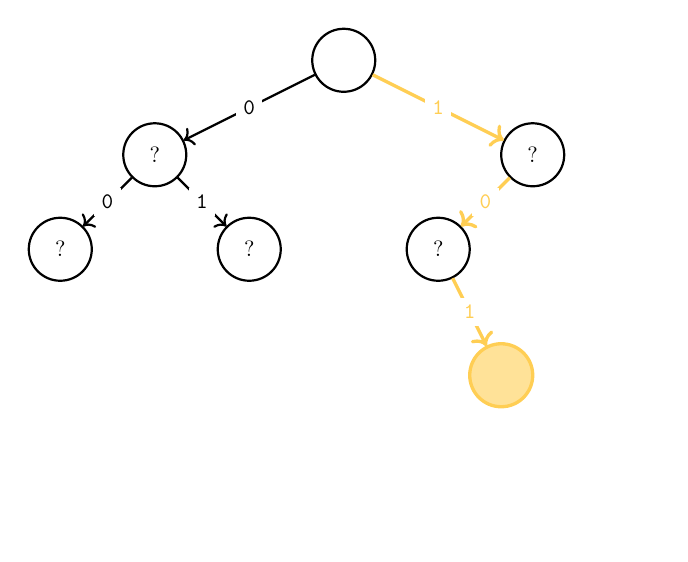
\begin{tikzpicture}[scale=0.8, transform shape]
      \node[defaultnode] (n1) at (0,0)  { $\varnothing$ };
      \node[defaultnode] (n2) at (-3,-1.5)  { ? };
      \node[defaultnode] (n3) at (3,-1.5)  { ? };
      \node[defaultnode] (n4) at (-4.5,-3)  { ? };
      \node[defaultnode] (n5) at (1.5,-3)  { ? };
      \node[defaultnode, opacity=0] (n7) at (4.5,-3)  { ? };
      \node[newnode] (n8) at (2.5,-5)  { $\varnothing$ };
      \node[defaultnode, opacity=0] (n9) at (2,-7)  { \texttt{k} };
      \node[defaultnode] (n6) at (-1.5,-3)  { ? };

      \draw[thick, ->] (n1) -- node[fill=white] {\texttt{0}} (n2);
      \draw[very thick, ->, myyellow] (n1) -- node[fill=white] {\texttt{1}} (n3);

      \draw[thick, ->] (n2) -- node[fill=white] {\texttt{0}} (n4);
      \draw[thick, ->] (n2) -- node[fill=white] {\texttt{1}} (n6);

      \draw[very thick, ->, myyellow] (n3) -- node[fill=white] {\texttt{0}} (n5);

      \draw[very thick, ->, myyellow] (n5) -- node[fill=white] {\texttt{1}} (n8);
      \draw[thick, ->, opacity=0] (n8) -- node[fill=white] {\texttt{0}} (n9);

    \end{tikzpicture}
  \end{center}
  \begin{center}
    \footnotesize\color{gray} traverse the edges based on the key's characters \\ attaching new nodes as needed
  \end{center}

\end{frame}

\begin{frame}
  \begin{center}
    \highlight{\textbf{insert}} \\
    \footnotesize\color{gray} \texttt{insert(1010, obj)}
  \end{center}
  \begin{center}

    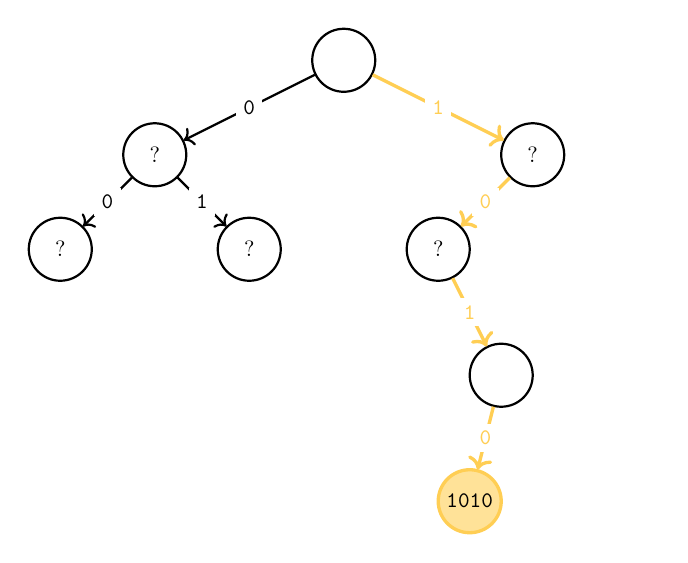
\begin{tikzpicture}[scale=0.8, transform shape]
      \node[defaultnode] (n1) at (0,0)  { $\varnothing$ };
      \node[defaultnode] (n2) at (-3,-1.5)  { ? };
      \node[defaultnode] (n3) at (3,-1.5)  { ? };
      \node[defaultnode] (n4) at (-4.5,-3)  { ? };
      \node[defaultnode] (n5) at (1.5,-3)  { ? };
      \node[defaultnode, opacity=0] (n7) at (4.5,-3)  { \texttt{1010} };
      \node[defaultnode] (n8) at (2.5,-5)  { $\varnothing$ };
      \node[newnode] (n9) at (2,-7)  { \texttt{1010} };
      \node[defaultnode] (n6) at (-1.5,-3)  { ? };

      \draw[thick, ->] (n1) -- node[fill=white] {\texttt{0}} (n2);
      \draw[very thick, ->, myyellow] (n1) -- node[fill=white] {\texttt{1}} (n3);

      \draw[thick, ->] (n2) -- node[fill=white] {\texttt{0}} (n4);
      \draw[thick, ->] (n2) -- node[fill=white] {\texttt{1}} (n6);

      \draw[very thick, ->, myyellow] (n3) -- node[fill=white] {\texttt{0}} (n5);

      \draw[very thick, ->, myyellow] (n5) -- node[fill=white] {\texttt{1}} (n8);
      \draw[very thick, ->, myyellow] (n8) -- node[fill=white] {\texttt{0}} (n9);

    \end{tikzpicture}
  \end{center}
  \begin{center}
    \footnotesize\color{gray} traverse the edges based on the key's characters \\ attaching new nodes as needed
  \end{center}
\end{frame}

\begin{frame}[fragile]
  \begin{proofbox}
    \begin{lstlisting}[style=mypython]
def insert(self: Trie, key: Key, obj: Object) -> Optional[TrieNode]:
    curr = self.root
    for char in key:
        if curr.children[char] is None:
            curr.children[char] = TrieNode()
            curr.children[char].pnt = curr
        curr = curr.children[char]
    curr.obj = obj
    self.size += 1
    return curr
\end{lstlisting}
  \end{proofbox}
\end{frame}


\begin{frame}
  \begin{center}
    \highlight{\textbf{delete}} \\
    \footnotesize\color{gray} \texttt{delete(10)}
  \end{center}
  \begin{center}

    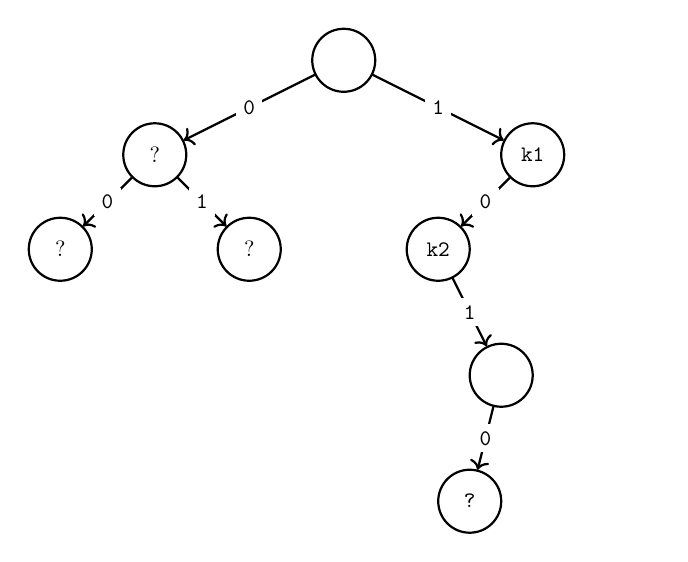
\begin{tikzpicture}[scale=0.8, transform shape]
      \node[defaultnode] (n1) at (0,0)  { $\varnothing$ };
      \node[defaultnode] (n2) at (-3,-1.5)  { ? };
      \node[defaultnode] (n3) at (3,-1.5)  { \texttt{k1} };
      \node[defaultnode] (n4) at (-4.5,-3)  { ? };
      \node[defaultnode] (n5) at (1.5,-3)  { \texttt{k2} };
      \node[defaultnode, opacity=0] (n7) at (4.5,-3)  { \texttt{k} };
      \node[defaultnode] (n8) at (2.5,-5)  { $\varnothing$ };
      \node[defaultnode] (n9) at (2,-7)  { \texttt{?} };
      \node[defaultnode] (n6) at (-1.5,-3)  { ? };

      \draw[thick, ->] (n1) -- node[fill=white] {\texttt{0}} (n2);
      \draw[thick, ->] (n1) -- node[fill=white] {\texttt{1}} (n3);

      \draw[thick, ->] (n2) -- node[fill=white] {\texttt{0}} (n4);
      \draw[thick, ->] (n2) -- node[fill=white] {\texttt{1}} (n6);

      \draw[thick, ->] (n3) -- node[fill=white] {\texttt{0}} (n5);

      \draw[thick, ->] (n5) -- node[fill=white] {\texttt{1}} (n8);
      \draw[thick, ->] (n8) -- node[fill=white] {\texttt{0}} (n9);

    \end{tikzpicture}
  \end{center}
  \begin{center}
    \footnotesize\color{gray} traverse the edges based on the key's characters \\ return if key not found
  \end{center}
\end{frame}

\begin{frame}
  \begin{center}
    \highlight{\textbf{delete}} \\
    \footnotesize\color{gray} \texttt{delete(10)}
  \end{center}
  \begin{center}

    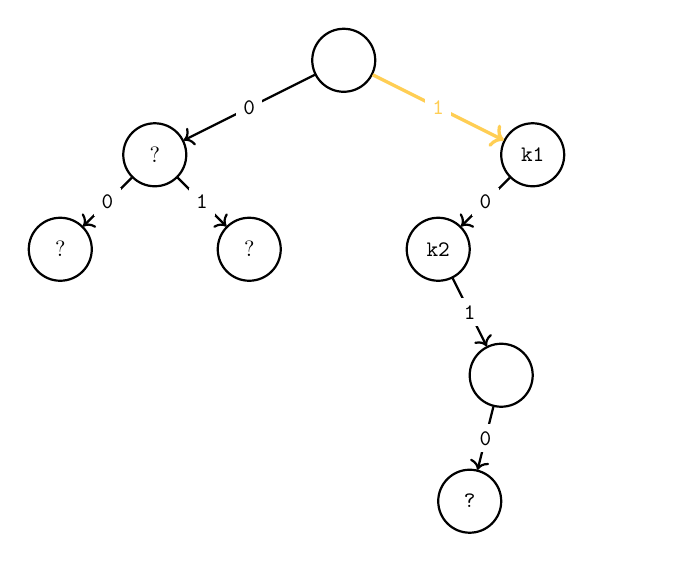
\begin{tikzpicture}[scale=0.8, transform shape]
      \node[defaultnode] (n1) at (0,0)  { $\varnothing$ };
      \node[defaultnode] (n2) at (-3,-1.5)  { ? };
      \node[defaultnode] (n3) at (3,-1.5)  { \texttt{k1} };
      \node[defaultnode] (n4) at (-4.5,-3)  { ? };
      \node[defaultnode] (n5) at (1.5,-3)  { \texttt{k2} };
      \node[defaultnode, opacity=0] (n7) at (4.5,-3)  { \texttt{k} };
      \node[defaultnode] (n8) at (2.5,-5)  { $\varnothing$ };
      \node[defaultnode] (n9) at (2,-7)  { \texttt{?} };
      \node[defaultnode] (n6) at (-1.5,-3)  { ? };

      \draw[thick, ->] (n1) -- node[fill=white] {\texttt{0}} (n2);
      \draw[very thick, ->, myyellow] (n1) -- node[fill=white] {\texttt{1}} (n3);

      \draw[thick, ->] (n2) -- node[fill=white] {\texttt{0}} (n4);
      \draw[thick, ->] (n2) -- node[fill=white] {\texttt{1}} (n6);

      \draw[thick, ->] (n3) -- node[fill=white] {\texttt{0}} (n5);

      \draw[thick, ->] (n5) -- node[fill=white] {\texttt{1}} (n8);
      \draw[thick, ->] (n8) -- node[fill=white] {\texttt{0}} (n9);

    \end{tikzpicture}
  \end{center}
  \begin{center}
    \footnotesize\color{gray} traverse the edges based on the key's characters \\ return if key not found
  \end{center}
\end{frame}


\begin{frame}
  \begin{center}
    \highlight{\textbf{delete}} \\
    \footnotesize\color{gray} \texttt{delete(10)}
  \end{center}
  \begin{center}

    \begin{tikzpicture}[scale=0.8, transform shape]
      \node[defaultnote] (n1) at (0,0)  { $\varnothing$ };
      \node[defaultnode] (n2) at (-3,-1.5)  { ? };
      \node[defaultnode] (n3) at (3,-1.5)  { \texttt{k1} };
      \node[defaultnode] (n4) at (-4.5,-3)  { ? };
      \node[defaultnode] (n5) at (1.5,-3)  { \texttt{k2} };
      \node[defaultnode, opacity=0] (n7) at (4.5,-3)  { \texttt{k} };
      \node[defaultnode] (n8) at (2.5,-5)  { $\varnothing$ };
      \node[defaultnode] (n9) at (2,-7)  { \texttt{?} };
      \node[defaultnode] (n6) at (-1.5,-3)  { ? };

      \draw[thick, ->] (n1) -- node[fill=white] {\texttt{0}} (n2);
      \draw[very thick, ->, myyellow] (n1) -- node[fill=white] {\texttt{1}} (n3);

      \draw[thick, ->] (n2) -- node[fill=white] {\texttt{0}} (n4);
      \draw[thick, ->] (n2) -- node[fill=white] {\texttt{1}} (n6);

      \draw[very thick, myyellow, ->] (n3) -- node[fill=white] {\texttt{0}} (n5);

      \draw[thick, ->] (n5) -- node[fill=white] {\texttt{1}} (n8);
      \draw[thick, ->] (n8) -- node[fill=white] {\texttt{0}} (n9);

    \end{tikzpicture}
  \end{center}
  \begin{center}
    \footnotesize\color{gray} traverse the edges based on the key's characters \\ return if key not found
  \end{center}
\end{frame}

\begin{frame}
  \begin{center}
    \highlight{\textbf{delete}} \\
    \footnotesize\color{gray} \texttt{delete(10)}
  \end{center}
  \begin{center}

    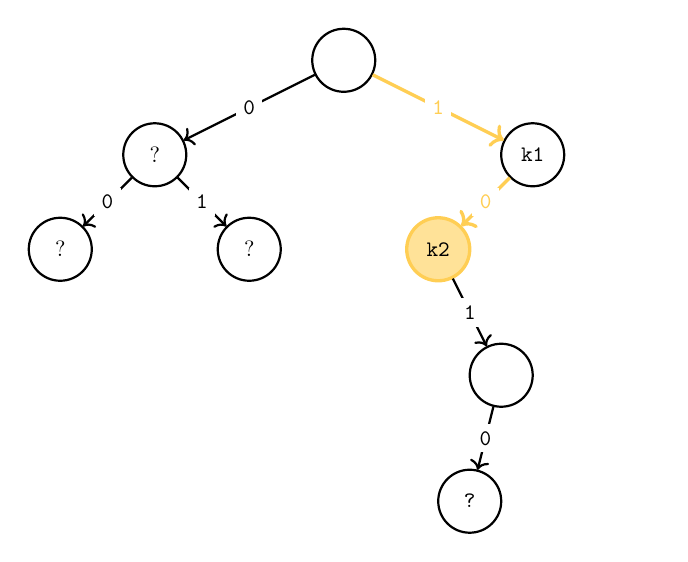
\begin{tikzpicture}[scale=0.8, transform shape]
      \node[defaultnode] (n1) at (0,0)  { $\varnothing$ };
      \node[defaultnode] (n2) at (-3,-1.5)  { ? };
      \node[defaultnode] (n3) at (3,-1.5)  { \texttt{k1} };
      \node[defaultnode] (n4) at (-4.5,-3)  { ? };
      \node[newnode] (n5) at (1.5,-3)  { \texttt{k2} };
      \node[defaultnode, opacity=0] (n7) at (4.5,-3)  { \texttt{k} };
      \node[defaultnode] (n8) at (2.5,-5)  { $\varnothing$ };
      \node[defaultnode] (n9) at (2,-7)  { \texttt{?} };
      \node[defaultnode] (n6) at (-1.5,-3)  { ? };

      \draw[thick, ->] (n1) -- node[fill=white] {\texttt{0}} (n2);
      \draw[very thick, ->, myyellow] (n1) -- node[fill=white] {\texttt{1}} (n3);

      \draw[thick, ->] (n2) -- node[fill=white] {\texttt{0}} (n4);
      \draw[thick, ->] (n2) -- node[fill=white] {\texttt{1}} (n6);

      \draw[very thick, myyellow, ->] (n3) -- node[fill=white] {\texttt{0}} (n5);

      \draw[thick, ->] (n5) -- node[fill=white] {\texttt{1}} (n8);
      \draw[thick, ->] (n8) -- node[fill=white] {\texttt{0}} (n9);

    \end{tikzpicture}
  \end{center}
  \begin{center}
    \footnotesize\color{gray} if the key is found, set the key to $\varnothing$ \\ \;
  \end{center}
\end{frame}

\begin{frame}
  \begin{center}
    \highlight{\textbf{delete}} \\
    \footnotesize\color{gray} \texttt{delete(10)}
  \end{center}
  \begin{center}

    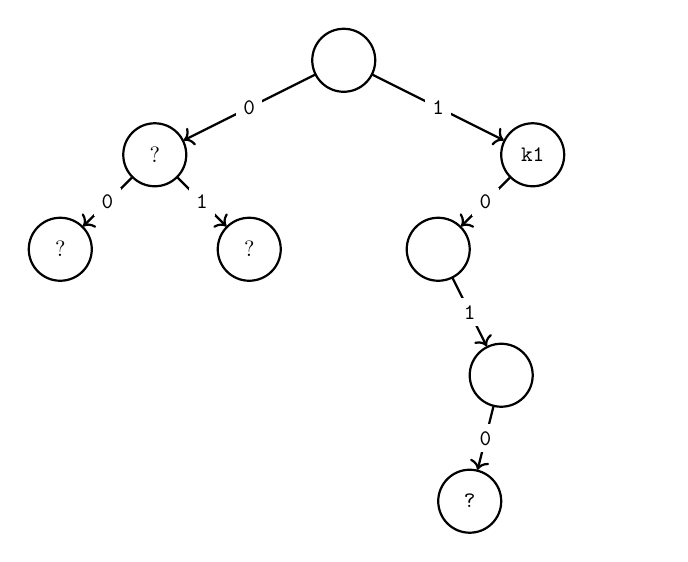
\begin{tikzpicture}[scale=0.8, transform shape]
      \node[defaultnode] (n1) at (0,0)  { $\varnothing$ };
      \node[defaultnode] (n2) at (-3,-1.5)  { ? };
      \node[defaultnode] (n3) at (3,-1.5)  { \texttt{k1} };
      \node[defaultnode] (n4) at (-4.5,-3)  { ? };
      \node[defaultnode] (n5) at (1.5,-3)  { $\varnothing$ };
      \node[defaultnode, opacity=0] (n7) at (4.5,-3)  { \texttt{k} };
      \node[defaultnode] (n8) at (2.5,-5)  { $\varnothing$ };
      \node[defaultnode] (n9) at (2,-7)  { \texttt{?} };
      \node[defaultnode] (n6) at (-1.5,-3)  { ? };

      \draw[thick, ->] (n1) -- node[fill=white] {\texttt{0}} (n2);
      \draw[thick, ->] (n1) -- node[fill=white] {\texttt{1}} (n3);

      \draw[thick, ->] (n2) -- node[fill=white] {\texttt{0}} (n4);
      \draw[thick, ->] (n2) -- node[fill=white] {\texttt{1}} (n6);

      \draw[thick, ->] (n3) -- node[fill=white] {\texttt{0}} (n5);

      \draw[thick, ->] (n5) -- node[fill=white] {\texttt{1}} (n8);
      \draw[thick, ->] (n8) -- node[fill=white] {\texttt{0}} (n9);

    \end{tikzpicture}
  \end{center}
  \begin{center}
    \footnotesize\color{gray} \; \\ \;
  \end{center}
\end{frame}



\begin{frame}[fragile]
  \begin{proofbox}
    \begin{lstlisting}[style=mypython]
def delete(self: Trie, key: Key) -> Optional[TrieNode]:
    def _delete(key: Key, curr: TrieNode, depth: Integer):
        if depth == len(key):
            if curr.children is empty:
                curr.pnt.children[key[depth-1]] = None
            else:
                curr.end = False
            return curr
        else:
            char = key[depth]
            if char in curr.children:
                should_prune = _delete(key, depth + 1)
        return not node.children and node.objue is None

    return _delete(self.root, key, 0)
\end{lstlisting}
  \end{proofbox}
\end{frame}

\begin{frame}
  Properties of the \texttt{Trie} data-structure:
  \begin{table}
    \begin{tabular}{@{} r | l @{} }
      \highlight{\textbf{Property}}            &                                  \\[1mm]\hline
      \multirow{1}{*}{Time Complexity}         &                                  \\
      \color{gray}\footnotesize\texttt{insert} & \color{gray}\footnotesize $O(L)$ \\[1mm]
      \color{gray}\footnotesize\texttt{get}    & \color{gray}\footnotesize $O(L)$ \\[1mm]
      \color{gray}\footnotesize\texttt{delete} & \color{gray}\footnotesize $O(L)$ \\[1mm]
      Space Complexity                         & $O(N)$
    \end{tabular}
  \end{table}
  \begin{center}
    \footnotesize\color{gray} properties of the \texttt{Trie} data-structure
  \end{center}
  \renewcommand\thefootnote{}\footnotetext{\color{gray} Assumptions: $N = $ \texttt{Trie.size}, $L = $ \texttt{len(key)}, where \texttt{key} is the longest}
\end{frame}


\begin{frame}{Appendix (Proofs)}
  \begin{center}
    \Large \highlight{\textbf{appendix}} \\[1mm]
    \normalsize \color{gray} (proofs)
  \end{center}
\end{frame}

\begin{frame}
  \begin{thmbox}
    The time complexity of \texttt{get} for the \texttt{Trie} (via Binary Search Trees) is $O(L)$, where $L = $ \texttt{len(key)} and $\texttt{key}$ is the longest.
  \end{thmbox}
  \begin{proofbox}
    \highlightc{lightgray}{\textbf{traversing the trie}}: \hfill $O(L)$ \\[1mm]
    \footnotesize\color{gray}
    Starting from the root, we follow the edges of the trie corresponding to each character in the key.
    For a fixed alphabet size, finding the appropriate edge for a character takes $O(1)$ time (using an array).
    If an edge does not exist, the key does not exist, so we stop early.  Otherwise, if all $L$ edges have been traversed, we return the key of the last node, which takes $O(1)$ time.
  \end{proofbox}
\end{frame}

\begin{frame}
  \begin{thmbox}
    The time complexity of \texttt{insert} in a \texttt{Trie} (via Binary Search Trees) is $O(L)$, where $L = \texttt{len(key)}$ and $\texttt{key}$ is the longest.
  \end{thmbox}
  \begin{proofbox}
    \highlightc{lightgray}{\textbf{traversing the trie}}: \hfill $O(L)$ \\[1mm]
    \footnotesize\color{gray}
    Starting from the root, we follow the edges of the trie corresponding to each character in the key.
    For a fixed alphabet size, finding the appropriate edge for a character takes $O(1)$ time (using an array).
    If an edge does not exist, attaching a new node also takes $O(1)$ time.
  \end{proofbox}
\end{frame}

\begin{frame}
  \begin{thmbox}
    The time complexity of \texttt{delete} for the \texttt{Trie} (via Binary Search Trees) is $O(L)$, where $L = $ \texttt{len(key)} and \texttt{key} is the longest.
  \end{thmbox}
  \begin{proofbox}
    \highlightc{lightgray}{\textbf{traversing the trie}}: \hfill $O(L)$ \\[1mm]
    \footnotesize\color{gray}
    Starting from the root, we follow the edges of the trie corresponding to each character in the key.
    For a fixed alphabet size, finding the appropriate edge for a character takes $O(1)$ time (using an array).
    If an edge does not exist, the key does not exist, so we stop early. Otherwise, if all $L$ edges have been traversed, we set the key of the last node to \texttt{NULL}, which takes $O(1)$ time.
  \end{proofbox}
\end{frame}

\end{document}